LLVM has emerged as the de-facto standard compiler infrastructure for modern software development, powering everything from the development environment for Apple operating systems to cutting-edge systems research efforts. Its adoption by the compiler community can be attributed to several key strengths---a modular architecture that separates language frontends from optimization backends, an extensive suite of analysis and transformation passes that expose deep insights into program behavior, and robust support for over 30 programming languages, including those supported by PythonTutor. LLVM even provides users with an API to define their own language \cite{LLVM2004}.

At the core of LLVM's value proposition for code analysis is its Intermediate Representation, a low-level and platform-independent format that captures program semantics in a standardized way. This IR serves as the foundation for powerful built-in analysis passes that can generate control flow graphs, dominator trees, data flow analyses, and detailed memory access patterns. For compiler developers and researchers, these capabilities are invaluable---LLVM effectively solves the hard problem of extracting structured information from code, allowing them to focus on higher-level tasks like optimization or verification \cite{LLVMRef}.

However, LLVM's visualization capabilities tell a different story. The standard approach for visualizing analysis results relies on generating DOT\footnote{A plain-text graph description language used by Graphviz to define nodes and edges for rendering graphs.} files through passes like \texttt{-dot-cfg} or \texttt{-view-cfg}, which are then rendered using Graphviz\cite{graphviz}. While functionally correct, the resulting diagrams---an example of which is shown in Fig.~\ref{fig:cfg}---embody a strictly utilitarian aesthetic: monochrome nodes and edges, densely packed labels filled with LLVM IR instructions, and layouts optimized for completeness rather than clarity. This ``function over form'' philosophy serves well enough as a developer tool for debugging optimizer passes, but it fails as a solution for communication beyond that narrow domain.

\begin{figure*}[htbp]
\centerline{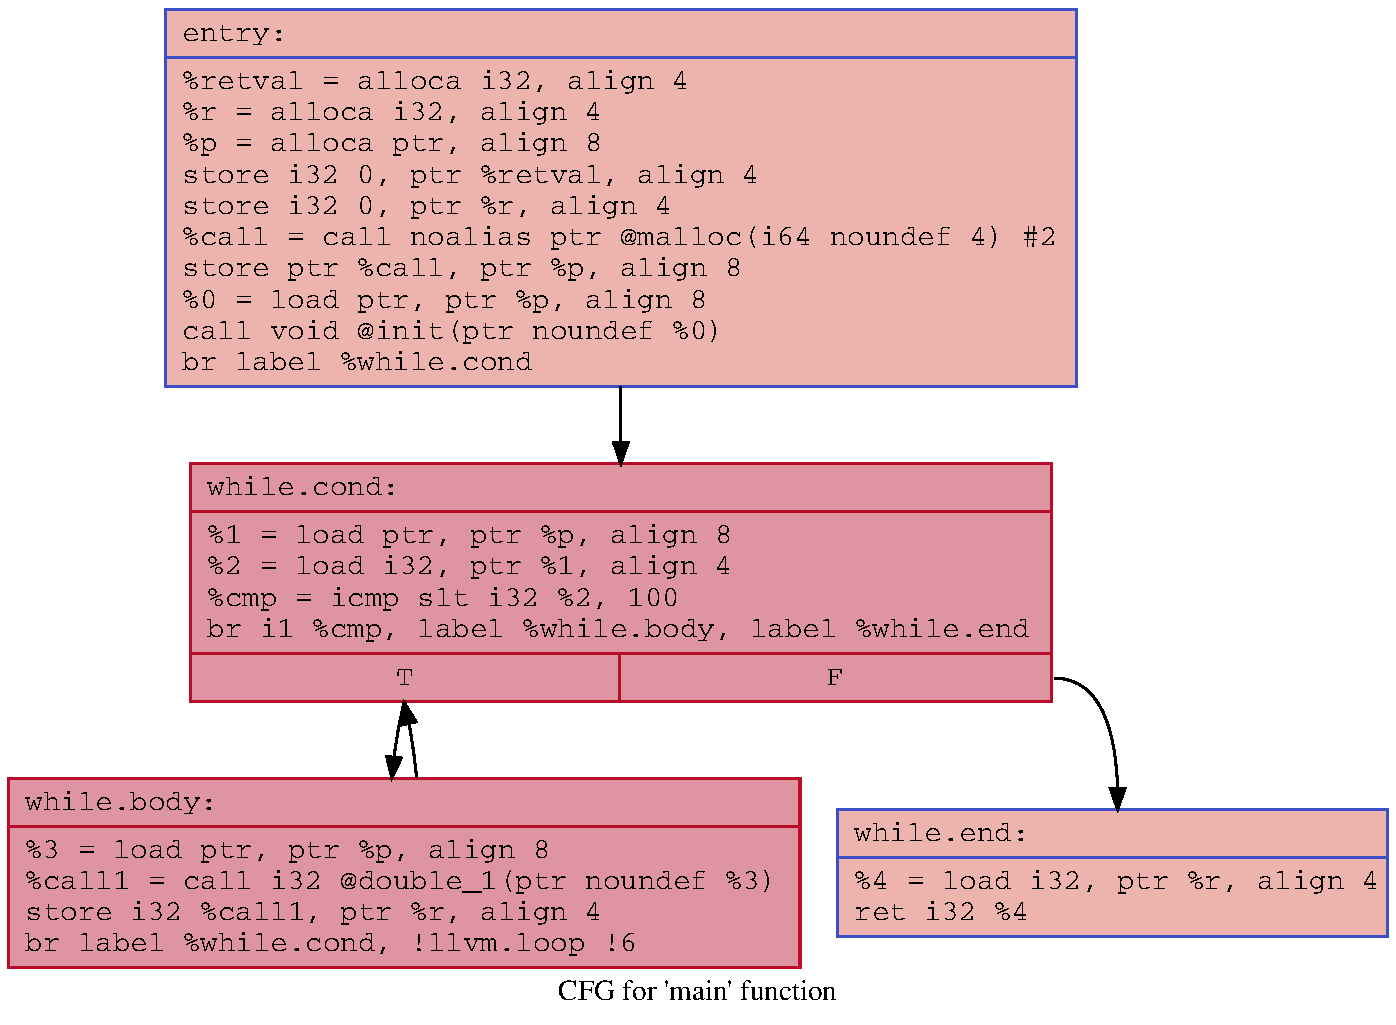
\includegraphics[width=0.75\textwidth]{images/CFG.pdf}}
\caption{Example Control-Flow Graph (CFG) using LLVM \texttt{-dot-cfg} pass. While technically accurate, the visualization prioritizes information density over visual clarity.}
\label{fig:cfg}
\end{figure*}

The barrier extends beyond mere aesthetics. Interpreting these diagrams requires familiarity with LLVM IR syntax---understanding what ``\texttt{\%4 = load i32, i32* \%3}'' means demands compiler knowledge that most audiences lack. The visualizations are fundamentally static images with no mechanism for progressive disclosure or animation, forcing presenters to mentally simulate execution flow while pointing at a frozen graph. Moreover, customization options are severely limited; changing colors, adjusting layouts, or highlighting specific execution paths requires manual post-processing in external tools, completely defeating the purpose of automated generation.

In essence, LLVM provides extraordinarily powerful analysis capabilities but pairs them with visualization tools that assume their primary consumer is someone who already understands what they are looking at. This creates a frustrating gap: rich semantic information about program behavior can be automatically extracted, but it cannot be automatically presented in a way that serves educational or presentational contexts. LLVManim was built to bridge this gap by maintaining LLVM's analytical rigor while replacing its austere output with animations designed for human communication rather than machine precision.
